\section{Emotions}
An important subject in the study of games is the emotions felt by the players. In MDA they feature as one of the three fundamental components of games. Emotions are traditionally a subject of psychology, but there are many studies focusing on emotions for games such as \cite{dillon_way_2010,bateman_implicit_2015,angelides_empirical_2014,karpouzis_emotion_2016}. This section covers baseline studies, on both games and psychology, meant to understand such complex subject and provide structure to this ontology.

There is no single line of research for emotions in psychology, however there are two major ways of studying them. One is called \textit{appraisal theory}, which consider emotions generated by appraisal and arousal, a valenced reaction to such appraisal \citep{ortony1990cognitive,scherer_appraisal_2001}. The other studies emotions as intrinsic manifestations, that is, there are a set of emotions understood as basic emotions which are natural to humans and independent of cultures and backgrounds, henceforth named \textit{basic emotion theory} \citep{ekman_are_basic_emotions_nodate,ekman_what_scientist_agree_2016}.

It is not in the scope of this work to discuss different psychological theories of emotions, or why and how they happen. What is of interest to this work is some structural model which exposes and classifies emotions that can be used as a basis for this ontology. That said, the appraisal theory models are more difficult to comprehend as they delve deeper in the terms of psychology and cognition. Whilst the basic emotion ones are simpler, much of this is due to the fact that appraisal theories are not about emotion words, that is, they do not intend to define emotion as they are used in common language. On the other hand, basic emotion theories study emotion from a perspective which focus on how the person interpret their own emotions and thus naturally it is defined in emotion words. 

The intention of this ontology is to be used by game designers and other persons interested in games, who do not necessarily have a deep knowledge of psychology. Basic emotions was then chosen as the theoretical foundation for the ontology of aesthetics because of its simplicity. The remainder of this section address two different models of basic emotions.

\subsection{Basic emotion models}

The following sections evaluates two different perspectives in basic emotion theory. One, built by \cite{dillon_way_2010}, is focused in the study of games, and therefore of great interesst to this work. The other one is a widely accepted and central theory created by \cite{ekman_are_basic_emotions_nodate}. Dillon's theory is not incompatible with Ekman's, actualy he uses the psychological theories of emotion created by many authors which agree with Ekman, and even use his theory. Thus this section analyzes two different takes on emotions studies, one purely psychological and the other applied to games, to find out how they can contribute to understanding emotions in games.

Also, it is important to make a clarification on basic emotions. This classification of an emotions in basic ones, is not in the sense that they are elements combined to create a more complex emotion, it denotes emotions which have a biological basis. The meaning behind this biological basis is that ``emotions are a product of our evolution" \cite{ekman_are_basic_emotions_nodate}. 

\subsection{The Atlas of Emotions}

Ekman created an atlas to illustrate his model which can be accessed at \url{http://atlasofemotions.org/} as of december 2018, it is the amalgamation of many years of research in emotions. This theory created by Ekman stands upon the assertion that emotions can be associated with physical reactions, to him, facial expressions.

The atlas identifies five basic emotions, anger, fear, disgust, sadness and enjoyment. Inside each basic emotion there are several emotional states, which are the ways a given person experiences this emotion. Each emotional state has its own intensity zone of the basic emotion it is related, this is illustrated by \autoref{fig:emotionalstates}. This zone represent how intense must be the emotion for the emotional state be manifested. Some of those states has zones that overlap, and can be felt at the same time. It is this conjunction of emotional states that represents the complexity of human emotion.

\begin{figure}[!h]
\hspace*{-1.25cm}
    \begin{tabular}{cc}
    
        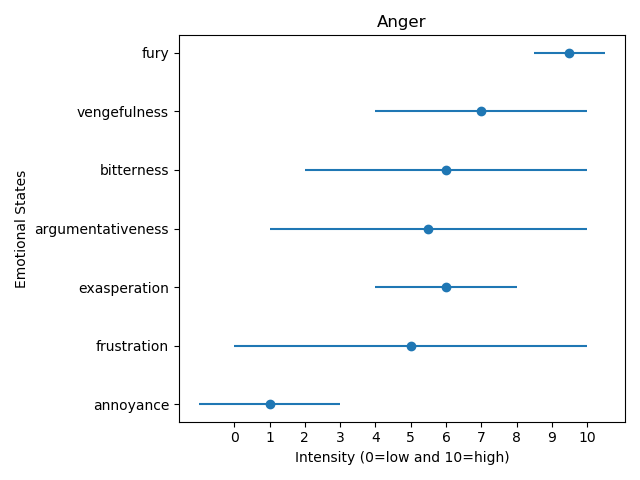
\includegraphics[scale=0.5]{Images/AtlasEmotionalStatesGraphics/Figure_anger.png} & 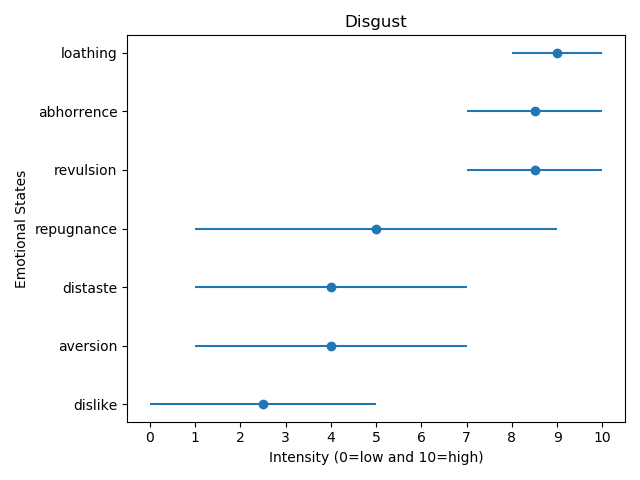
\includegraphics[scale=0.5]{Images/AtlasEmotionalStatesGraphics/Figure_Disgust.png} \\
        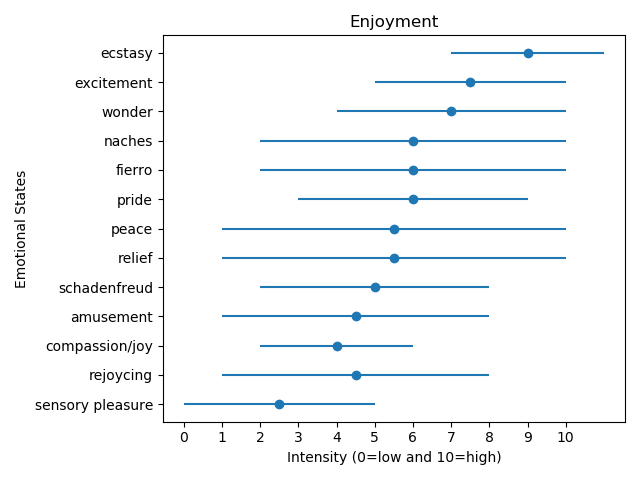
\includegraphics[scale=0.5]{Images/AtlasEmotionalStatesGraphics/Figure_Enjoyment.png} & 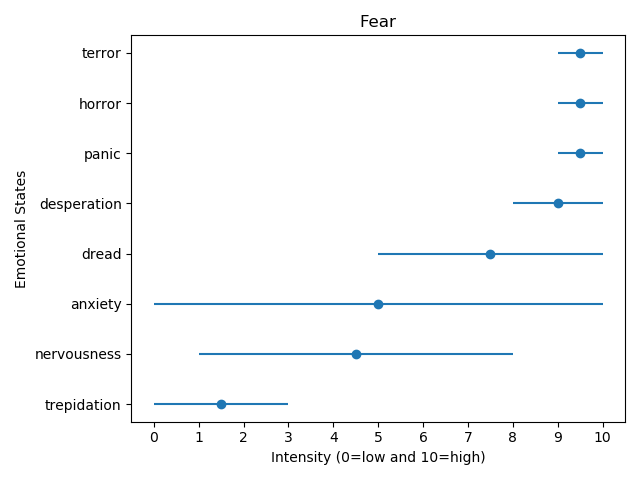
\includegraphics[scale=0.5]{Images/AtlasEmotionalStatesGraphics/Figure_Fear.png} \\
        \multicolumn{2}{c}{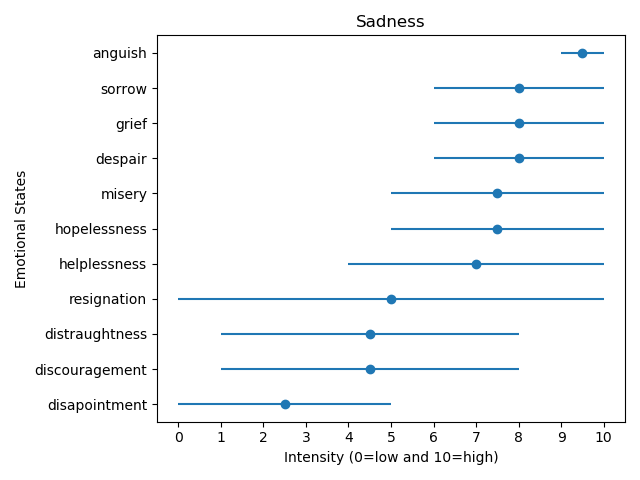
\includegraphics[scale=0.5]{Images/AtlasEmotionalStatesGraphics/Figure_Sadness.png}}
    \end{tabular}
    
    \caption{Emotional States intensity}
    \label{fig:emotionalstates}
\end{figure}


Common responses in each emotional states are also identified in Ekman's model. They evaluate the usual reactions a person express when feeling a particular emotion state. There is also present the notion of mood, a mood is a mental state which causes a particular emotion to be more likely felt. 

\subsection{The 6-11 model}

In his book \textit{On the way to fun} \citeauthor{dillon_way_2010} tackles the challenge of studying game design using emotions as his main perspective. His work consists of looking at successful games, that is, games which had a great acceptance of the public and received lots of positive criticism analyzing the emotions those games evoke. With this analysis Dillon creates a framework to understand how emotions behave in games, which is called 6-11.

6-11 stands as the name of the framework because this model is structured around 6 basic emotions and 11 instincts. The 6 emotions are fear, anger, pride, excitement, sadness and joy and the 11 instincts, survival, identification, collecting
, greed, aggressiveness, revenge, competition, protection/care, curiosity, communication, color appreciation are related as according to the framework diagram in \autoref{fig:611_diag}. The solid lines relates emotions to instincts they evoke and dashed lines instinct to the emotions they cause. Relations between emotions and between instincts appear in Dillon's book, but are not thoroughly explored by him. Most important are the relations between emotions and instincts. Thus for clarity of information relations between concepts of the same kind were left out of the diagram. 

%6-11 diagram
\begin{figure}[ht!]
\centering

\begin{tikzpicture}[squarednode/.style={rectangle, 
					rounded corners, 
					very thick,
 					minimum width=3cm,
					minimum height=1cm,
					draw=black!80, 
					fill=red!10},
					squarednode2/.style={rectangle, 
					rounded corners, 
					very thick,
 					minimum width=3cm,
					minimum height=1cm,
					draw=black!80, 
					fill=blue!10}
					]
					
% To reduce all image, transform canvas
% forgets about image size, so 
% we need a bounding box
% This is lame, but works with Eduardo Thesis´s image (now black and white for elegance)

% don´t ask me about theses limits
% I just tried until I found which ones
%workded

\useasboundingbox (3,-8) rectangle (8,9);
\scope[transform canvas={scale=1}]
         % Your actual drawing


%emotion nodes
\node[squarednode]  (emo1) [anchor = west, yshift = 7cm ] {Fear};
\node[squarednode]  (emo2) [below of = emo1, node distance=2cm, anchor=north] {Anger};
\node[squarednode]  (emo3) [below of = emo2, node distance=2cm, anchor=north] {Pride};
\node[squarednode]  (emo4) [below of = emo3, node distance=2cm, anchor=north] {Excitement};
\node[squarednode]  (emo5) [below of = emo4, node distance=2cm, anchor=north] {Sadness};
\node[squarednode]  (emo6) [below of = emo5, node distance=2cm, anchor=north] {Joy};

% instinct nodes
\node[squarednode2]  (inst1) [right of = emo1, node distance = 6cm, anchor = west, yshift = 1.5cm]{Survival};
\node[squarednode2]  (inst2) [below of = inst1, node distance=1cm, anchor=north] {Identification};
\node[squarednode2]  (inst3) [below of = inst2, node distance=1cm, anchor=north] {Collecting};
\node[squarednode2]  (inst4) [below of = inst3, node distance=1cm, anchor=north] {Greed};
\node[squarednode2]  (inst5) [below of = inst4, node distance=1cm, anchor=north] {Aggressiveness};
\node[squarednode2]  (inst6) [below of = inst5, node distance=1cm, anchor=north] {Revenge};
\node[squarednode2]  (inst7) [below of = inst6, node distance=1cm, anchor=north] {Competition};
\node[squarednode2]  (inst8) [below of = inst7, node distance=1cm, anchor=north] {Protection/Care};
\node[squarednode2]  (inst9) [below of = inst8, node distance=1cm, anchor=north] {Curiosity};
\node[squarednode2]  (inst11) [below of = inst9, node distance=1cm, anchor=north] {Color Appreciation};
\node[squarednode2]  (inst10) [below of = inst11, node distance=1cm, anchor=north] {Communication};


% Arrows Emo to Inst
\path[-latex, black, very thick] (emo1.east) edge  coordinate[midway](c_to_m) (inst1.west);

\path[-latex, black, very thick] (emo2.east) edge  coordinate[midway](c_to_m) (inst5.west);

\path[-latex, black, very thick] (emo2.east) edge  coordinate[midway](c_to_m) (inst6.west);

\path[latex'-latex', black, very thick] (emo3.east) edge  coordinate[midway](c_to_m) (inst7.west);

%arrows Inst to Emo
%survival
\path[-latex, dashed, black, very thick] (inst1.west) edge  coordinate[midway](c_to_m) (emo2.east);
\path[-latex, dashed, black, very thick] (inst1.west) edge  coordinate[midway](c_to_m) (emo5.east);
%Identification
\path[-latex, dashed, black, very thick] (inst2.west) edge  coordinate[midway](c_to_m) (emo1.east);
\path[-latex, dashed, black, very thick] (inst2.west) edge  coordinate[midway](c_to_m) (emo2.east);
\path[-latex, dashed, black, very thick] (inst2.west) edge  coordinate[midway](c_to_m) (emo3.east);
\path[-latex, dashed, black, very thick] (inst2.west) edge  coordinate[midway](c_to_m) (emo4.east);
\path[-latex, dashed, black, very thick] (inst2.west) edge  coordinate[midway](c_to_m) (emo5.east);
%Collecting
\path[-latex, dashed, black, very thick] (inst3.west) edge  coordinate[midway](c_to_m) (emo3.east);
%Greed
\path[-latex, dashed, black, very thick] (inst4.west) edge  coordinate[midway](c_to_m) (emo4.east);
%agressivenes
\path[-latex, dashed, black, very thick] (inst5.west) edge  coordinate[midway](c_to_m) (emo4.east);
%revenge
\path[-latex, dashed, black, very thick] (inst6.west) edge  coordinate[midway](c_to_m) (emo4.east);
% Competition
\path[-latex, dashed, black, very thick] (inst7.west) edge  coordinate[midway](c_to_m) (emo4.east);
\path[-latex, dashed, black, very thick] (inst7.west) edge  coordinate[midway](c_to_m) (emo2.east);
%Protection/care
\path[-latex, dashed, black, very thick] (inst8.west) edge  coordinate[midway](c_to_m) (emo2.east);
\path[-latex, dashed, black, very thick] (inst8.west) edge  coordinate[midway](c_to_m) (emo3.east);
\path[-latex, dashed, black, very thick] (inst8.west) edge  coordinate[midway](c_to_m) (emo5.east);
\path[-latex, dashed, black, very thick] (inst8.west) edge  coordinate[midway](c_to_m) (emo6.east);
%curiosity
\path[-latex, dashed, black, very thick] (inst9.west) edge  coordinate[midway](c_to_m) (emo1.east);
\path[-latex, dashed, black, very thick] (inst9.west) edge  coordinate[midway](c_to_m) (emo4.east);
%communication
\path[-latex, dashed, black, very thick] (inst10.west) edge  coordinate[midway](c_to_m) (emo4.east);
\path[-latex, dashed, black, very thick] (inst10.west) edge  coordinate[midway](c_to_m) (emo6.east);
%color apreciation
\path[-latex, dashed, black, very thick] (inst11.west) edge  coordinate[midway](c_to_m) (emo6.east);

% Inter concepts
% Emotions

\draw [->, line width=0.5mm, dotted] (emo3.west) -- ([xshift= -1cm]emo3.west) -- ([xshift=-1cm]emo6.west) -- (emo6.west);

%Instincts

\draw [->, line width=0.5mm, dotted] (inst1.east) -- ([xshift= 0.5cm]inst1.east) -- ([xshift=0.5cm]inst5.east) -- (inst5.east);

\draw [->, line width=0.5mm, dotted] (inst2.east) -- ([xshift= 0.75cm]inst2.east) -- ([xshift=0.75cm,yshift = 0.2cm]inst9.east) -- ([yshift = 0.2cm]inst9.east);

\draw [->, line width=0.5mm, dotted] (inst2.east) -- ([xshift= 0.75cm]inst2.east) -- ([xshift=0.65cm]inst8.east) -- (inst8.east);

\draw [->, line width=0.5mm, dotted] (inst3.south)  -- (inst4.north);

\draw [->, line width=0.5mm, dotted] (inst4.south)  -- (inst5.north);

\draw [->, line width=0.5mm, dotted] (inst6.north)  -- (inst5.south);

\draw [->, line width=0.5mm, dotted] (inst5.east) -- ([xshift= 0.25cm]inst5.east) -- ([xshift=0.25cm]inst7.east) -- (inst7.east);

\draw [->, line width=0.5mm, dotted] (inst9.east) -- ([xshift= 1cm]inst9.east) -- ([xshift=01cm]inst3.east) -- (inst3.east);

\draw [->, line width=0.5mm, dotted] (inst11.north)  -- (inst9.south);

\draw [<->, line width=0.5mm, dotted] (inst10.east) -- ([xshift= 1.25cm]inst10.east) -- ([xshift=1.25cm]inst2.east) -- (inst2.east);

    \endscope
\end{tikzpicture}
\caption{6-11 model Diagram}
\label{fig:611_diag}
\end{figure}

Differently from the Atlas of emotions, Dillon's identifies 6 basic emotions. Some of them very akin o those of the atlas while others even feature in the atlas as emotional states. That said, the emotions section of the 6-11 framework is very similar to the emotions proposed by Ekman and there is no novelty remark to be made.

Instincts are introduced by this model. Dillon does not give a precise definition of instincts as ``the analysis of instincts can spur disagreement among sociologists and psychologists''\citep{dillon_way_2010}. Instead he provides some common accepted characteristics of instincts:
\begin{itemize}
    \item Are automatic
    \item Are irresistible
    \item Occur at some point in development
    \item Are triggered by some event in the environment
    \item Occur in every member of the species
    \item Cannot be modified
    \item Govern a behavior for which the organism needs no 
training
\end{itemize}

Upon this he states that for this model's purpose the focus lies upon the fact that instincts are triggered by some event in the environment and that ``we can simply take the others for granted and let sociologists debate over them.''\citep{dillon_way_2010}. Which means that the framework models not what or why such instincts are present in games, but how they happen.

The last part of the 6-11 framework is how each emotion relates to each instinct. This is a causal relation, when a given emotion evokes a certain instinct or a instinct triggers a particular emotion. The purpose of this relation is to be possible to analyze how those two concepts interacts within a game. How a given emotion is felt by the player and what is responsible for this feeling, and which consequences this emotion brings to him. 
